\begin{frame}
    \centering
    \begin{figure}[H]
        
\includegraphics[keepaspectratio, width=0.7\paperwidth, height=\paperheight]{Logos/LeeLogo}
    \end{figure}
    Informatik: Programmieren\\
    \emoji{abacus} Kapitel 3:  \textbf{Zeit-Tabellen}
\end{frame}

% command to make sure colorboxes don't create whitespace between code lines
\fboxsep=.6pt

% default settings for listings
\lstset{style=python, basicstyle=\scriptsize\ttfamily,escapechar=!}


\begin{frame}[fragile]{Wo lebt eine Variable? \emoji{house}}

\begin{minipage}[c]{.6\linewidth}
\begin{lstlisting}
import turtle as t

def quadrat(seitenlaenge):
    for _ in range(4):
        !\only<1-4,6-8>{t.forward(seitenlaenge)}
          \only<5,9->{t.forward(\colorbox{CarnationPink}{seiten\tikzmark{arrowFrom3a}laenge})}!
        t.right(90)

def quadrat_muster(aktuelle_seitenlaenge):
    for _ in range(50):
        !\only<1-2,5,6,9->{quadrat(aktuelle\_seitenlaenge)}
        \only<3,7>{quadrat(\colorbox{CarnationPink}{aktuelle\_\tikzmark{arrowFrom2a}seitenlaenge})}
        \only<4,8>{\colorbox{CarnationPink}{quadrat(aktuelle\_\tikzmark{arrowFrom2}seitenlaenge)}}!
        !\only<1-5,7->{aktuelle\_seitenlaenge += 3}
        \only<6>{\colorbox{CarnationPink}{aktuelle\_sei\tikzmark{arrowFrom4a}tenlaenge += 3}}!
        
!\only<1,3->{quadrat\_muster(30)}
\only<2>{\colorbox{CarnationPink}{quadrat\tikzmark{arrowFrom1}\_muster(30)}}!
\end{lstlisting}
\end{minipage}
\begin{minipage}[c]{.37\linewidth}
    \only<1>{
\begin{figure}[H]
\centering
        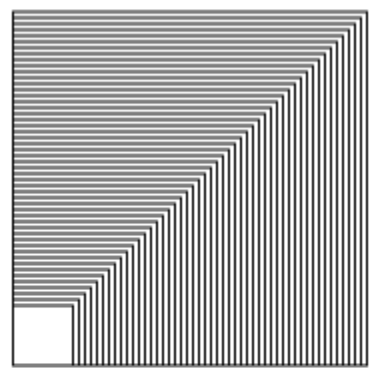
\includegraphics[width=.75\linewidth]{Grundlagen_Info/00_Programmieren/Figures/prog-8-squares.png}
    \end{figure}}
    \only<4->{
\begin{table}[H]
    \centering
    \scriptsize
    
    \begin{tabular}{c|c}
         \rowcolor{LightCyan}Variable & Wert \\\midrule\midrule
         \lstinline|seitenlaenge| & \tikzmark{arrowTo3a}\only<1-7>{\lstinline|30|}\only<8->{33}
    \end{tabular}
\caption*{\tikzmark{arrowBbox2Start}\lstinline|quadrat|\tikzmark{arrowBbox2End}}
\end{table}}
    \only<2->{
    \begin{table}[H]
            \centering
            \scriptsize
            \begin{tabular}{c|c}
                 \rowcolor{LightCyan} Variable & Wert \\\midrule\midrule
                 \lstinline|aktuelle_seitenlaenge| & \tikzmark{arrowTo2a}\only<1-5>{\lstinline|30|}\only<6->{33}
                 
            \end{tabular}
            \caption*{\tikzmark{arrowBbox1Start}\lstinline|quadrat_muster|\tikzmark{arrowBbox1End}}
        \end{table}
    }
\end{minipage}


\begin{tikzpicture}[overlay,remember picture]
\only<2>{
       % Draw a 2D rectangle around the table title
        \node[fit=(arrowBbox1Start) (arrowBbox1End), inner sep=4pt, red, dotted, draw, line width=1pt,rounded corners](dottedRect1) {};
        
        % draw arrow to title
    \draw[red,-stealth] (arrowFrom1.north) to[bend right] node[right, fill=RoyalBlue,text=white,rounded corners] {\tiny Tabelle erstellen} (dottedRect1);    

    }
   \only<3,7>{
   % nachschlagen
           \draw[red,-stealth] (arrowFrom2a.north) to[bend right] node[right, fill=RoyalBlue,text=white,rounded corners] {\tiny Nachschlagen} (arrowTo2a);    }
\only<4,8>{
           % Draw a 2D rectangle around the table title
            \node[fit=(arrowBbox2Start) (arrowBbox2End), inner sep=4pt, red, dotted, draw, line width=1pt,rounded corners](dottedRect2) {};
            
            % draw arrow to title
        \draw[red,-stealth] (arrowFrom2.north) to[bend right] node[right, xshift=.3cm, yshift=1cm, fill=RoyalBlue,text=white,rounded corners] {\tiny Tabelle erstellen} (dottedRect2);    
    }
   \only<5,9>{
   % nachschlagen
           \draw[red,-stealth] (arrowFrom3a.north) to[bend right] node[right, fill=RoyalBlue,text=white,rounded corners] {\tiny Nachschlagen} (arrowTo3a);    }
           
    \only<6>{
       % Wert aktualisieren
               \draw[red,-stealth] (arrowFrom4a.north) to[bend right] node[right, fill=RoyalBlue,text=white,rounded corners] {\tiny Wert aktualisieren} (arrowTo2a);    }
\end{tikzpicture}
\normalsize
\only<10->{
\begin{itemize}
\item Bei jedem Aufruf einer \lstinline|def| wird eine Tabelle erstellt, die die Namen und Werte aller Parameter enthält
\item Parameter sind sogenannte \enquote{\textbf{lokal}} und existieren nur innerhalb einer Definition
\end{itemize}
}
\end{frame}

\begin{frame}[fragile]{Übungen}
\begin{itemize}
    \item \aufgabebox{Aufgaben 3.35 - 3.39}
    \item \abgabebox{Abgabe (Moodle): Aufgabe 3.38}
\end{itemize}
\end{frame}